\documentclass[a4paper,11pt]{article}
\usepackage[utf8]{inputenc}
\usepackage{lastpage}
\usepackage{fancyhdr}
\usepackage[english]{babel}
\usepackage[a4paper,left=1in,right=1in,top=1in,bottom=.9in]{geometry}
\usepackage{multirow}
\usepackage[table,xcdraw,dvipsnames]{xcolor}
\usepackage{array}
\usepackage{amsmath}
\usepackage{graphicx}
\usepackage{caption}
\usepackage{ctable}
\usepackage{listings}


\graphicspath{ {images/} }

\newcolumntype{L}[1]{>{\raggedright\let\newline\\\arraybackslash\hspace{0pt}}m{#1}}
\newcolumntype{C}[1]{>{\centering\let\newline\\\arraybackslash\hspace{0pt}}m{#1}}
\newcolumntype{R}[1]{>{\raggedleft\let\newline\\\arraybackslash\hspace{0pt}}m{#1}}

\newcommand\tab[1][4mm]{\hspace*{#1}}


%-------------------------------------------------------------------------------
% HEADER & FOOTER
%-------------------------------------------------------------------------------

\pagestyle{fancy}
\fancyhf{}
\setlength\headheight{15pt}
\fancyhead[L]{ HPC Assignment 3 }
\fancyhead[R]{Student ID: 100633486}
\fancyfoot[R]{Page \thepage\ of \pageref{LastPage}}


%-------------------------------------------------------------------------------
% TITLE PAGE
%-------------------------------------------------------------------------------

\begin{document}

\title{
	\Huge \textbf {Langevin Dynamics, Part II}
    \\ [0.2cm]
	\LARGE HPC Assignment 3 - March, 2017
    \\ [0.5cm]
    \hrule
}

\date{}

\author{
		\Large Kamyar Nazeri \\
		\large Student ID: 100633486 }

\maketitle
\newpage

\section*{Introduction}
In this assignment, we are simulating the Langevin dynamics, making the code that utilizes interactions thread-parallel and analysing the output data. \\
These specifications have been incorporated into our simulation model:
\begin{itemize}
  \item Particle trajectories are implemented in 2D.
  \item Equation is equipped with periodic boundary conditions.
  \item OpenMP \cite{omp} library is used to execute the code in parallel.
  \item Lennard-Jones potential model \cite{lj} is used to approximate the interaction between a pair of particles.
\end{itemize}

\section*{C++ Data Structure}
The C++ code base for this assignment contains data-structures that represent Particle, Sector and Neighbor entities. Program procedures like ordering particles, assigning particles to a sector, and iterating over sectors are performed using arrays of aforementioned data-structures. The class diagram of the data-structures used in our program is shown in \emph{Figure 1}:

\begin{figure}[!htb]
  \centering
  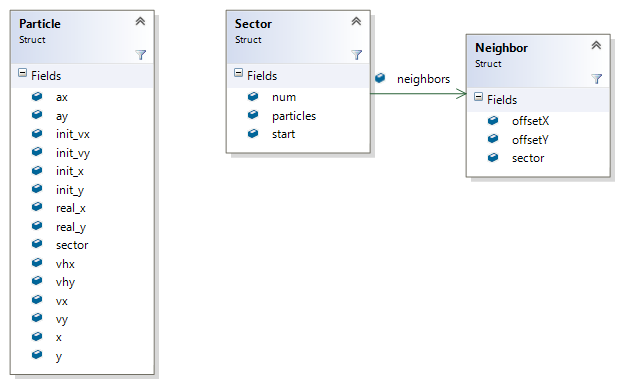
\includegraphics{class_diagram.png}
  \caption{\small Class diagram: Particle, Sector, Neighbor}
\end{figure}
\begin{itemize}
    \setlength\itemsep{0em}
\item \emph{Particle} struct contains the values for initial position, real position, position, initial velocity, velocity, velocity verlet, acceleration and the corresponding sector.
\item \emph{Sector} struct contains the number of the sector in typewriter index, starting index of the particles, number of the particles and an array of its \emph{Neighbors}
\item \emph{Neighbor} struct contains the index of a sector and its offset with the declaring sector when considering boundary condition.
\end{itemize}
\newpage

\section*{Pseudo-Code}
\begin{itemize}
\item\textbf{Pseudo-Code for the main loop (over time-steps):} \\
\bgroup\obeylines\small
initialize time to zero: $time = 0$ \\

WHILE time \(<\) total time
    \tab FOR all particles $\rightarrow$ \textbf{p}
        \tab\tab calculate particle's velocity verlet: $vh = velocity + \frac{1}{2} (acceleration \times \Delta t)$
        \tab\tab calculate particle's position: $position = position + vh \times \Delta t$
    \tab ENDFOR \\

    \tab CALL \emph{impose-boundary-condition} function passing array of particles
    \tab CALL \emph{order} function to order the particles positions by sector, passing particles and sectors
    \tab CALL \emph{random-number-generator} function to create a normally distributed random force: $\rightarrow \eta$
    \tab remove number of particles in the dumpster from the actual particles count \\

    \tab FOR all particles $\rightarrow$ \textbf{p}
    \tab\tab reset particle's acceleration: $acceleration = 0$
    \tab\tab calculate particle's acceleration using the random force: $ acceleration = \frac{1}{m}(-\gamma v + \frac{\sqrt{2\gamma k_B T}}{\sqrt{\Delta t}}\eta) $
    \tab ENDFOR \\

    \tab FOR all sectors $\rightarrow$ \textbf{sec}
        \tab\tab FOR all particles in the sector \emph{sec} $\rightarrow$ \textbf{p}
            \tab\tab\tab FOR all neighbors of the sector \emph{sec} $\rightarrow$ \textbf{nbr}
                \tab\tab\tab\tab FOR all particles in the neighbor \emph{nbr} $\rightarrow$ \textbf{np}
                    \tab\tab\tab\tab\tab calculate the distance between \emph{p} and \emph{np} + offset of the neighboring sector $\rightarrow$ \textbf{dist}
                    \tab\tab\tab\tab\tab IF dist $<$ range of interaction
                        \tab\tab\tab\tab\tab\tab calculate the force using Lennard-Jones potential \cite{lj} $\rightarrow$ \textbf{F}
                        \tab\tab\tab\tab\tab\tab calculate the acceleration using the interaction force: $acceleration = \frac{acceleration \times F}{m}$
                    \tab\tab\tab\tab\tab ENDIF
                \tab\tab\tab\tab ENDFOR
            \tab\tab\tab ENDFOR
        \tab\tab ENDFOR
    \tab ENDFOR \\

    \tab FOR all particles $\rightarrow$ \textbf{p}
        \tab\tab calculate the velocity: $velocity = vh + \frac{1}{2} (acceleration \times \Delta t)$
    \tab ENDFOR \\

    \tab update time iteration: $time = time + \Delta t$
ENDWHILE
\egroup

\newpage
\item\textbf{Pseudo-Code for neighbor-list subroutine:}
\bgroup\obeylines\small
LET \textbf{d} = linear number of sectors, \textbf{L} = domain size
FOR all sectors $\rightarrow$ \textbf{sec}
    \tab get sector's typewriter index $\rightarrow$ \textbf{index}
    \tab compute the chess-board indices from the sector's typewriter index $\rightarrow$ \textbf{row, col}
    \tab FOR $nrow = row - 1$ to $row + 1$
        \tab\tab FOR $ncol = col - 1$ to $col + 1$
            \tab\tab\tab calculate the neighbor sector's offset when imposing boundary condition:
            \tab\tab\tab\tab left \& top: -L, right \& bottom: L
            \tab\tab\tab\tab $offsetX = (round(\frac{ncol + d}{d}) - 1) \times L$
            \tab\tab\tab\tab $offsetY = (round(\frac{nrow + d}{d}) - 1) \times L$
            \tab\tab\tab calculate the neighboring sector index from the chessboard indices:
            \tab\tab\tab\tab $neighboring \ sector\ index = (nrow \times d) + ncol$
        \tab\tab ENDFOR
    \tab ENDFOR
ENDFOR \\
\egroup

\item\textbf{Pseudo-Code for order and assign subroutine:}
\bgroup\obeylines\small
LET \textbf{d} = linear number of sectors, \textbf{L} = domain size, \textbf{width} = $\frac{L}{d}$
LET \textbf{particles} = array of all particles
FOR all particles $\rightarrow$ \textbf{p}
    \tab IF particle's position is in the domain: $p.x < \frac{L}{2}$ and $p.y < \frac{L}{2}$
        \tab\tab assign a sector index to the particle: $p.sector = \frac{p.y + \frac{L}{2}}{width} \times d + \frac{p.x + \frac{L}{2}}{width}$
        \tab\tab keep count of all particles in the sector: $sector.particles = sector.particles + 1$
    \tab ELSE
        \tab\tab put the particle outside bounds in dumpster: $p.sector = d \times d$
        \tab\tab keep count of all particles in the dumpster: $dumpster.particles = dumpster.particles + 1$
    \tab ENDIF
ENDFOR \\

LET $sum = 0$
FOR all sectors $\rightarrow$ \textbf{sec}
    \tab set sector's start index to sum of all particles in previous sectors: $sec.start = sum$
    \tab calculate sum of all previous particles: $sum = sum + sec.particles$
    \tab reset number of particles in the sector prior ordering: $sec.particles = 0$
ENDFOR \\

LET $copy = particles$
FOR all particles in \textbf{\emph{copy}} $\rightarrow$ \textbf{p}
    \tab find p's sector $\rightarrow$ \textbf{sec}
    \tab reorder the array of all particles by placing all particles with the same sector together:
    \tab\tab $particles[sec.start + sec.particles] = p$
    \tab keep count of all particles in the sector: $sec.particles = sec.particles + 1$
ENDFOR

\egroup
\end{itemize}

\newpage
\section*{Particles Initialization}
When taking into account the interaction force between particles, the initial positions for the particles must not lead to excessive interaction forces. This requirement must hold even if the density of the particles is large.\\
In this assignment, we implement the initialization by drawing a mesh from all possible positions the particles can take on in the domain without interaction. We define an array of all those positions and use the \emph{Fisher–Yates algorithm} \cite{fy} to shuffle this array. To initialize \emph{n} particles, we draw the first \emph{n} elements from the shuffled array. \emph{Figure 2} represents this implementation in 3 stages. From left to right: draw a mesh, shuffle the array, take first \emph{n} elements.
\begin{figure}[!htb]
  \centering
  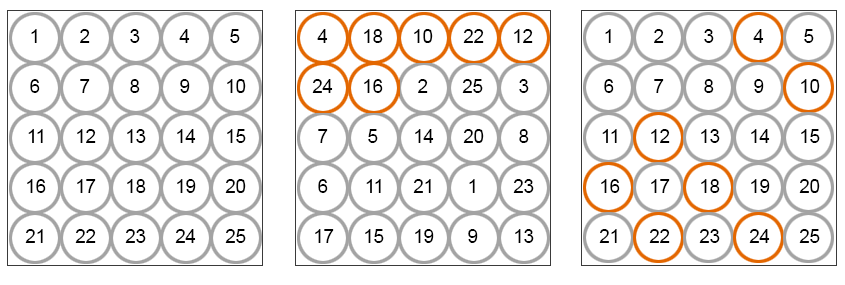
\includegraphics[width=16cm, height=5.4cm]{init.png}
  \caption{\small Random initialization of 7 particles in a domain than contains up to 25 particles}
\end{figure}
\section*{Finding best time step}
In our simulation, values of variables are changed at distinct, separate ``points in time", meaning time is viewed as a discrete variable. Thus, a non-time variable (position) jumps from one value to another as time moves from one time period to the next. This could lead to an increase in the number of particles escaping the domain due to the repelling force between the particles stepping onto each other. To fix this issue, one can set the time-step small enough so that no particle could jump more than the ``interaction radius" in one time step. Using the velocity-verlet to calculate particle's change in position, we can find the minimum value for $dt$:
\begin{align*}
  \frac{1}{2}\frac{F}{m}dt^2 < rc \tab \Rightarrow \tab dt < \sqrt{\frac{2m\ rc}{F}}
\end{align*}
Where $rc$ is the interaction radius, $dt$ is the time-step, $m$ is the particle's mass and $F$ is a random force in the original Langevin equation. The following table shows the number the particles stepping onto each other (lost from the domain) for different values of time-step. As the time-step becomes smaller, fewer particles step onto each other. (from the equation above, for $m=1$ and $sigma=0.1$ we expect $dt$ to be less than 0.03)
\begin{center}
\emph{Particles(n): 40,000 \tab Domain Size(L): 100 \tab Range of Interaction(sigma): 0.1}
\end{center}

\begin{center}
\setlength\extrarowheight{2pt}\small
\begin{tabular}{|C{2cm}|C{2cm}|C{2cm}|C{5cm}|}
\hline
Time Step & Iterations & Interactions & Lost Particles / Total Particles \\ \hline
1 s & 100 & 43676 & 19200 / 40000 \\ \hline
0.1 s & 100 & 98164 & 6393 / 40000 \\ \hline
0.01 s & 100 & 91054 & 754 / 40000 \\ \hline
0.001 s & 100 & 84520 & 0 / 40000 \\ \hline
\end{tabular}
\end{center}
\tab $\bullet$ time-step = 1 seconds, 19,200 particles escape the domain out of 43,676 interactions.\\
\tab $\bullet$ time-step = 0.001 seconds, no particles escape the domain out of 84,520 interactions.
\newpage

\section*{Root-Mean-Square Displacement}
To calculate the right root-mean-square displacement, we measure the deviation time between the position of a particle and its initial position:
\begin{align*}
  MSD \equiv \frac{1}{N}\sum_{n=0}^{N}(x_n(t) - x_n(0))^2 \tab \Rightarrow \tab RMS \equiv \sqrt{MSD}
\end{align*}
To measure the \emph{MSD} we have to keep track of each particle's initial position. This means in the \emph{Particle} data structure, we need to save the \emph{initial} position of each particle. Also, to have a continuous displacement of a particle when it moves across the periodic boundaries, we need to save the \emph{real} position of the particles (without imposing the boundary conditions) in the \emph{Particle} data structure. The MSD is measured using the \emph{real} and \emph{initial} values. At each iteration, particles that leave the domain are put in the dumpster and removed from the calculation. \\
We are experiencing a spike in the mean-square displacement when the number of particles is relatively small. The spike happens almost when the particles start leaving the domain and they are put back in due to the boundary condition effect. The domain size in \emph{figure 4} is twice the size of the domain in \emph{figure 3}. Notice the spike in the MSD is happening almost twice as late. This is probably the result of the interaction force between the particles already inside the domain and those that are put back in due to imposing the boundary condition.

\begin{figure}[!htb]
    \centering
    \begin{minipage}{.5\textwidth}
      \centering
      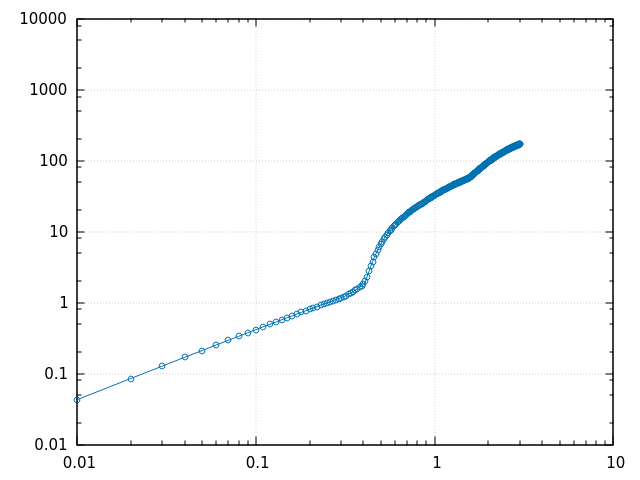
\includegraphics[width=7cm, height=4.5cm]{rms_n1000_l50.png}
      \caption{\small Particles: 1,000 \\ domain size: 50}
    \end{minipage}%
    \begin{minipage}{.5\textwidth}
      \centering
      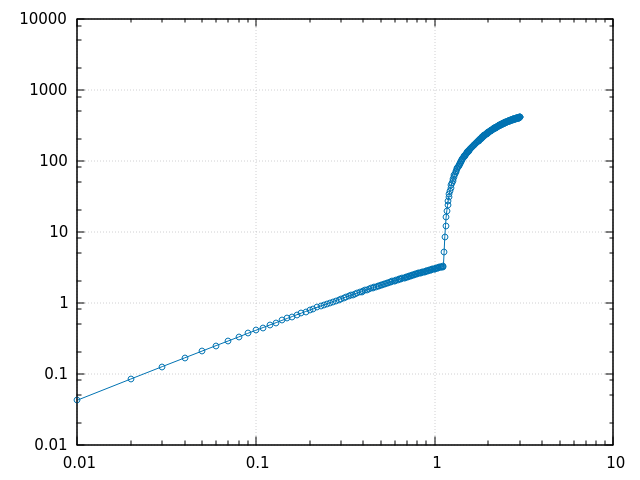
\includegraphics[width=7cm, height=4.5cm]{rms_n1000_l100.png}
      \caption{\small Particles: 1,000 \\ domain size = 100}
    \end{minipage}
\end{figure}

\noindent On the other hand, when the domain size is so large (\emph{figure 5}) that no particle can leave the domain, or when there is a relatively large number of particles in the domain (\emph{figure 6}) so that many particles experience the interaction force at each time-step, the ballistic-diffusive regimes are similar to the one without the interaction force and there's no spike in the MSD:
\begin{figure}[!htb]
    \centering
    \begin{minipage}{.5\textwidth}
      \centering
      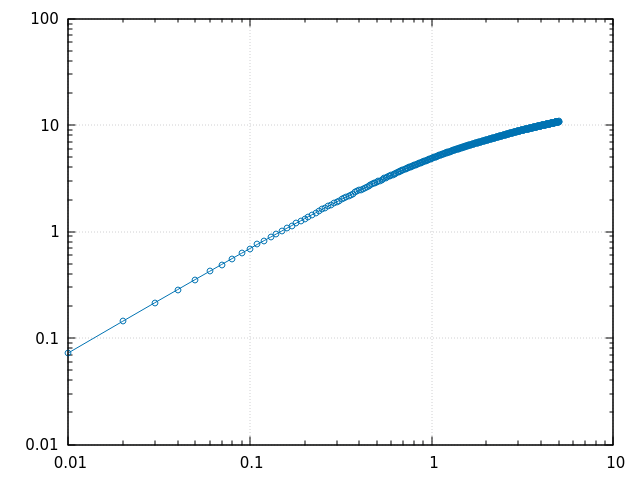
\includegraphics[width=7cm, height=4.7cm]{rms_n1000_l1000.png}
      \caption{\small particles: 1,000 \\ domain size: \textcolor{red}{1,000}}
    \end{minipage}%
    \begin{minipage}{.5\textwidth}
      \centering
      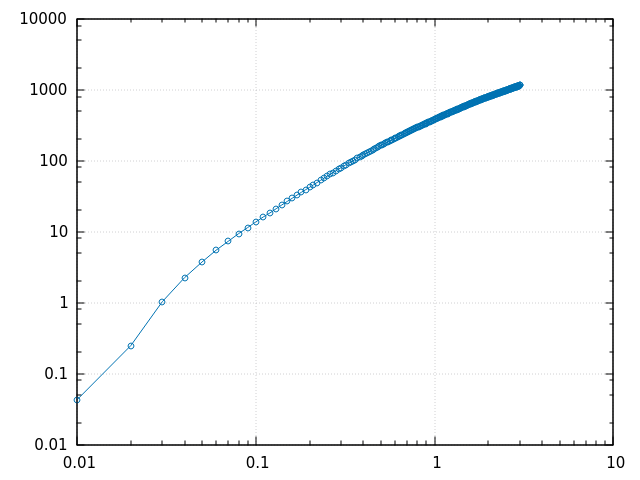
\includegraphics[width=7cm, height=4.7cm]{rms_n4000_l100.png}
      \caption{\small particles = \textcolor{red}{40,000} \\ domain size: 100}
    \end{minipage}
\end{figure}

\newpage

\section*{Parallelization \& Domain Composition}
We use OpenMP \cite{omp} library to make the code thread-parallel. The pragma \emph{omp parallel for} is used to fork additional threads to carry out the work for computation of the interactions. In addition, to increase the program performance, we use \emph{domain composition} to assign the particles to sectors based on their positions. Each sector in the domain composition has 8 neighboring sectors. To compute the interaction force between particles, every particle in each sector will be compared with only the particles in the neighboring sectors. The following table shows the effect of parallelism and domain composition on the wall-time:

\begin{center}
\emph{Particles(n): 40,000 \tab Domain Size(L): 100 \tab Range of Interaction(sigma): 0.1}
\end{center}

\begin{center}
\setlength\extrarowheight{3.5pt}
\begin{tabular}{|C{3.1cm}|C{3cm}|C{3.3cm}|}
\hline
Linear Number of Sectors & Wall-Time (seconds) & Parallel Wall-Time (seconds) \\ \specialrule{.05em}{0em}{.03em}
3 & \cellcolor{red!20}{1008} & \textcolor{ForestGreen}{526} \\ \hline
5 & 205 & \textcolor{ForestGreen}{132} \\ \hline
10 & 51.2 & \textcolor{ForestGreen}{34.4} \\ \hline
20 & 13.2 & \textcolor{ForestGreen}{12.5} \\ \hline
100 & 4.2 & \textcolor{red}{6.8} \\ \specialrule{.05em}{0em}{.02em}
200 & \cellcolor{green!20}{4} & \textcolor{red}{6.6} \\ \hline
400 & 4.3 & \textcolor{red}{6.8} \\ \hline
800 & 5.7 & \textcolor{red}{8.1} \\ \hline
\end{tabular}
\end{center}

\section*{Efficiency of the domain composition:}
The minimum value for the linear number of sectors is 3 (i.e. 9 sectors), hence to simulate the serial, single domain implementation, one can choose the linear number of sectors to be 3. This means that each sector, together with its neighboring sectors, covers the whole domain, and, as a result, every particle is compared with all the particles in the domain. This leads to the worst program performance, and the biggest wall-time in our simulations: \textbf{1008 seconds}. \\
By increasing the number of sectors, the amount of wall-time decreases by a factor of $\frac{1}{d^2}$, with the best performance occurring around $\frac{n}{d^2}\approx1$ which, for uniformly distributed particles, means there's almost one particle in each sector. In our simulations, this happens with $d = 200$, which results in a wall-time of \textbf{4 seconds}. Greater values for \emph{d} mean that there are more sectors in the domain than the number of particles and would have a negative impact on the overall performance of the program.

\section*{Efficiency of the parallelization:}
The efficiency of the parallelism depends on two variables: (1) the total number of the cpu cores available (two cores in our test machine), and (2) the number of flops for a single iteration of all sectors ($9 \times \frac{n^2}{d^4}$). As demonstrated in the table above, parallelism shows its benefits only when the number of flops gets to the millions (e.g. $\approx$ \emph{23,000,000 flops} with \emph{d = 5}) and it starts to lose efficiency, with a decline in the number of flops. \\
We cannot implement the optimum domain composition and parallelism at the same time since they are mutually exclusive; and with only 2 physical cores in our test machine, thread-parallelism would not be desirable and domain composition remains the best option.

\newpage
\section*{Other time consuming tasks:}
Besides ``computation of the interactions", the only time consuming part of the program is writing data on the disk. Every other part of the program including ordering, imposing boundary conditions, calculating velocity and generating random numbers is of the order \emph{O(n)} and relatively fast. Our tests indicate that the amount of time required to write data on disk for 40,000 particles is almost 3.8 seconds, while the times required for ordering, imposing boundary condition, generating random numbers and calculating particle velocities are 0.41 seconds, 0.03 seconds, 0.03 seconds and 0.08 seconds respectively. This means that writing is the performance bottleneck, and even by exploiting parallel algorithms for these tasks, one cannot expect much improvement in the overall value of the wall-time. \\
To make parts of the code run in parallel, we make use of the pragma \emph{omp parallel sections} to divide the work among separate threads. The sections we define to be run in parallel are: calculating the velocities, writing particle positions on disk, and writing MSD on the disk. The performance gain using parallel section in our tests with 40,000 particles is merely 0.4 seconds:

\begin{lstlisting}[basicstyle=\tiny,language=C++]
#pragma omp sections
{
    #pragma omp section
    {
        // calculate the velocities
    }

    #pragma omp section
    {
        // write particles positions on disk: trajectories
    }

    #pragma omp section
    {
        // write mean-square displacement on disk: means
    }
}
\end{lstlisting}

\section*{Influence of the interactions on the MSD:}
The influence of the interactions on the mean-square displacement is unclear with our simulations. As demonstrated in \emph{Figure 6}, when there is relatively a large number of particles in the domain so that many particles experience the interaction force at each time-step, the ballistic-diffusive regimes are similar to the one without the interaction force. \\
However, the influence of the interactions on the velocities of the particles is distinct, as more interactions between particles means an increase in the velocity of the particles. The distribution of the velocities of particles is demonstrated in the following figures. Note that the distribution of the velocities becomes more spread out (\emph{Figure 8}) when we incorporate the interaction force into the equation:

\begin{figure}[!htb]
    \centering
    \begin{minipage}{.5\textwidth}
      \centering
      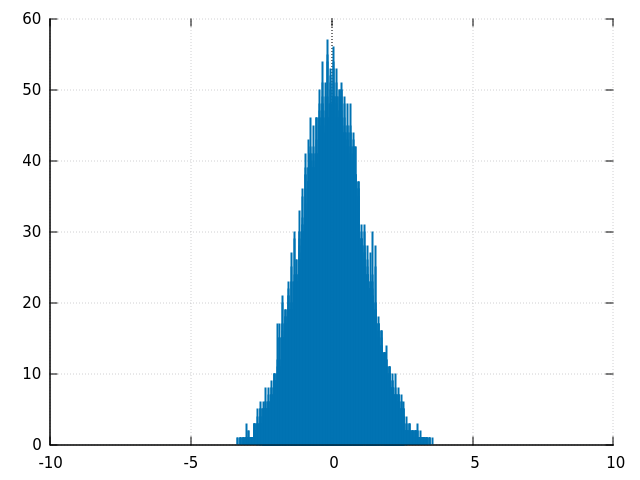
\includegraphics[width=7cm, height=5.25cm]{vel_non_inter.png}
      \caption{\small Velocity distribution \\ no interaction}
    \end{minipage}%
    \begin{minipage}{.5\textwidth}
      \centering
      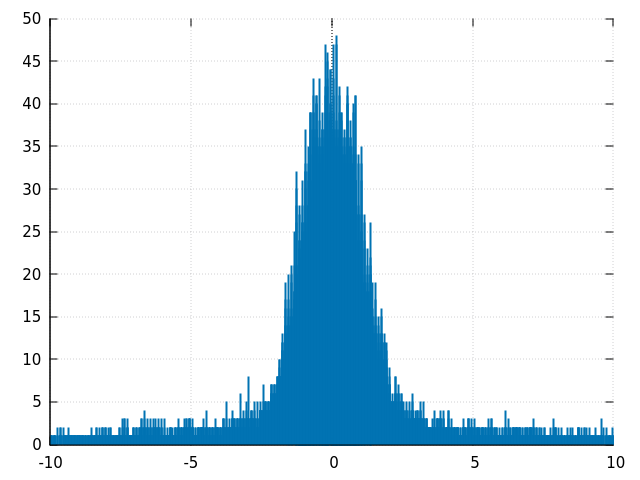
\includegraphics[width=7cm, height=5.25cm]{vel_inter.png}
      \caption{\small Velocity distribution \\ with interaction}
    \end{minipage}
\end{figure}

\newpage

\begin{thebibliography}{9}

\bibitem{omp}
The OpenMP API specification for parallel programming,
\\\texttt{http://www.openmp.org/resources/openmp-compilers/}

\bibitem{lj}
Lennard-Jones potential,
\\\texttt{https://en.wikipedia.org/wiki/Lennard-Jones\_potential}

\bibitem{fy}
Fisher–Yates shuffle algorithm,
\\\texttt{https://en.wikipedia.org/wiki/Fisher-Yates\_shuffle}

\end{thebibliography}

\end{document}
